\documentclass[border=1cm]{standalone}
\usepackage{tikz}
\usepackage{amsmath}
\begin{document}

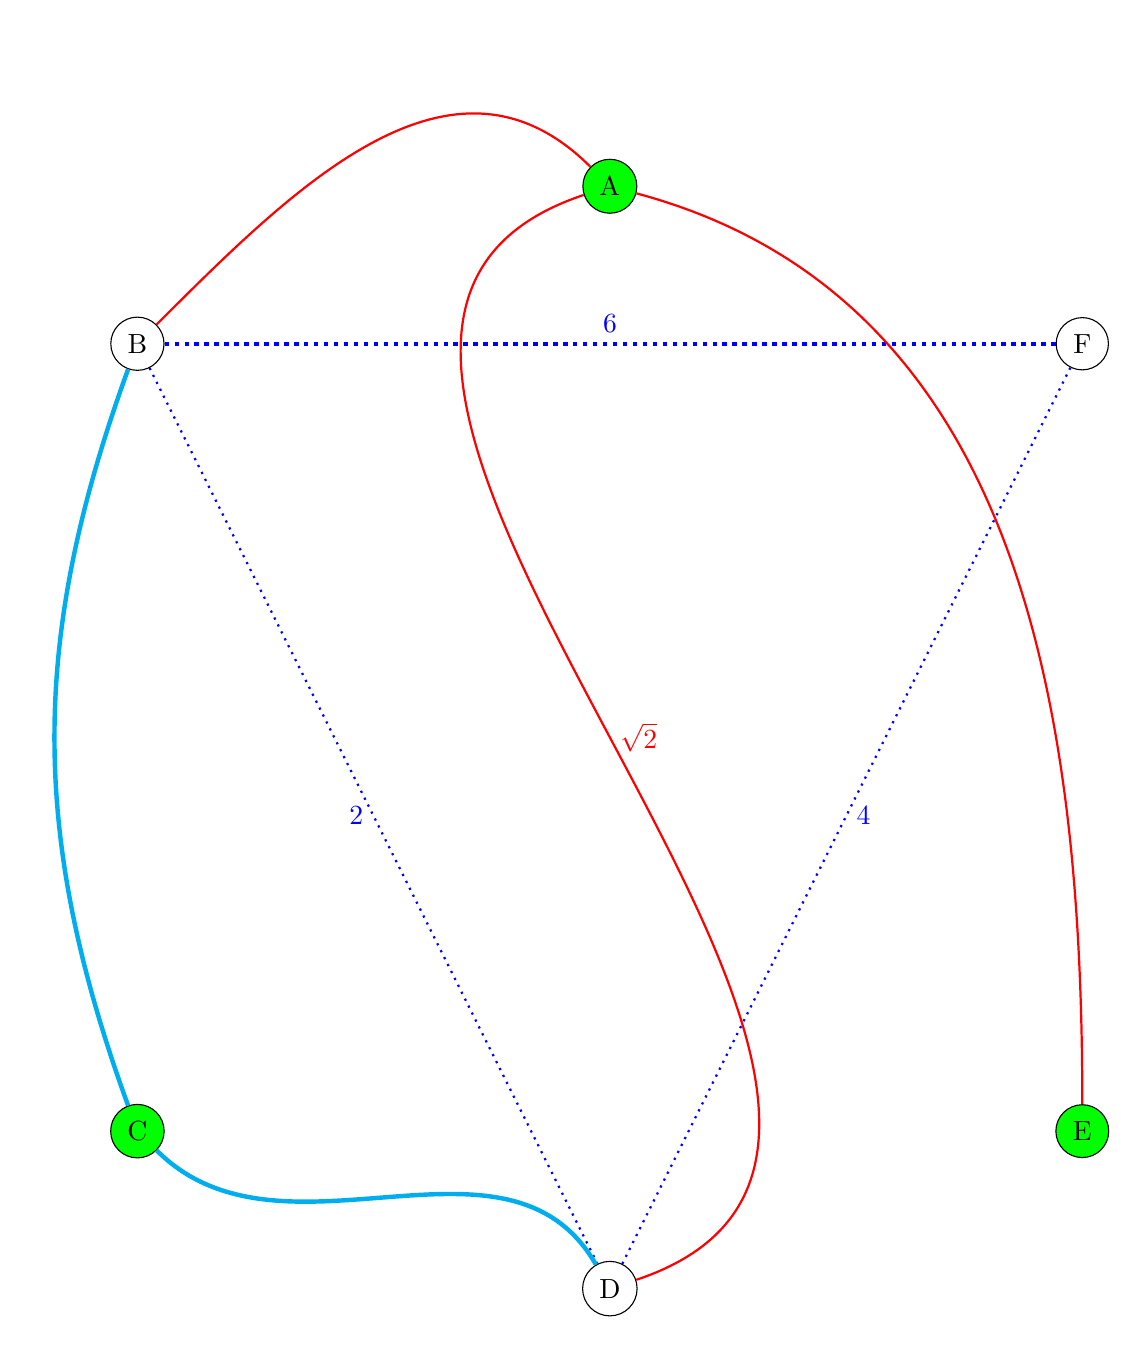
\begin{tikzpicture}[scale=2]
% Define the nodes
\node[circle, draw, fill=green] at (0,3) (a) {A};
\node[circle, draw, fill=green] at (-3,-3) (c) {C};
\node[circle, draw, fill=green] at (3,-3) (e) {E};
\node[circle, draw] at (3,2) (f) {F};
\node[circle, draw] at (-3,2) (b) {B};
\node[circle, draw] at (0,-4) (d) {D};
% Draw the paths
\draw[blue,dotted,ultra thick] (b) -- (f) node[midway, above]{6};
\draw[blue,dotted,thick] (b) -- (d) node[midway, above, left]{2};
\draw[blue,dotted,thick] (d) -- (f) node[midway, above, right]{4};
\draw[red,thick] (d) .. controls (3,-3) and (-3,2) .. (a) node[midway, above, right]{$\sqrt{2}$};
\draw[red,thick] (a) to[out=-15, in=90] (e);
\draw[red,thick] (b) .. controls (-2,3) and (-1,4) .. (a);
\draw[cyan,ultra thick] (b) to[out=-110, in=110]  (c);
\draw[cyan,ultra thick] (c) to[out=-45, in=120] (d);
\end{tikzpicture}

\begin{tikzpicture}[scale=2]
% Draw the x and y axis, label the axes and the origin
\draw[gray, ->] (-1,0) -- (2,0) node[right]{$x$} node[pos=0.33, below]{$O$};
\draw[gray, ->] (0,-2) -- (0,8) node[above]{$y$};
\draw[fill,gray] (0,0) circle [radius=1pt];
\draw (1,-0.05) -- (1,0.05) node[below, yshift=-2pt] {$x=1$};

% Plot the curve
\draw[blue, thick] [domain=-1:2, samples=150] plot (\x, {exp(\x)}) node[right]{$y = e^x$};
\draw[black, thick] [domain=0.1:2, samples=150] plot (\x, {ln(\x)}) node[right]{$y = ln(x)$};
% Note: the r in the argument of the cosine signifies that we enter \x in radians
\end{tikzpicture}

\end{document}